\section{Umsetzung}

\subsection{Datenbasis}

Als Grundlage dieser Arbeit wurde ein Korpus aus Texten von insgesamt 7 deutschsprachigen, der verschwörungstheoretiker Szene zuzurechnenden Internetangeboten erstellt.
\todo{R zitieren so nicht schon geschehen}
Die Skripte zum automatischen Abruf der Texte nutzen dafür das R-Paket \textit{rvest} \parencite{rvest} erstellt und extrahieren mittels für jede Seite seperat erstellten CSS-Selektoren und XPATH-Querys den jeweiligen Artikeltext. 
In diesem Vorgang wurden noch kleinere Bereinigungen an den Texten vorgenommen um wiederkehrende, nicht zum Artikeltext gehörende Elemente wie Werbung oder Spendenaufrufe zu entfernen, die Texte selbst wurden jedoch soweit möglich nicht weiter bearbeitet.
Weiterhin erfasst wurde zu den Artikeln das (angegebene) Veröffentlichungsdatum, der Artikeltitel sowie die Rubrik so diese Angabe vorhanden waren.

\begin{figure}[h]
    \centering
    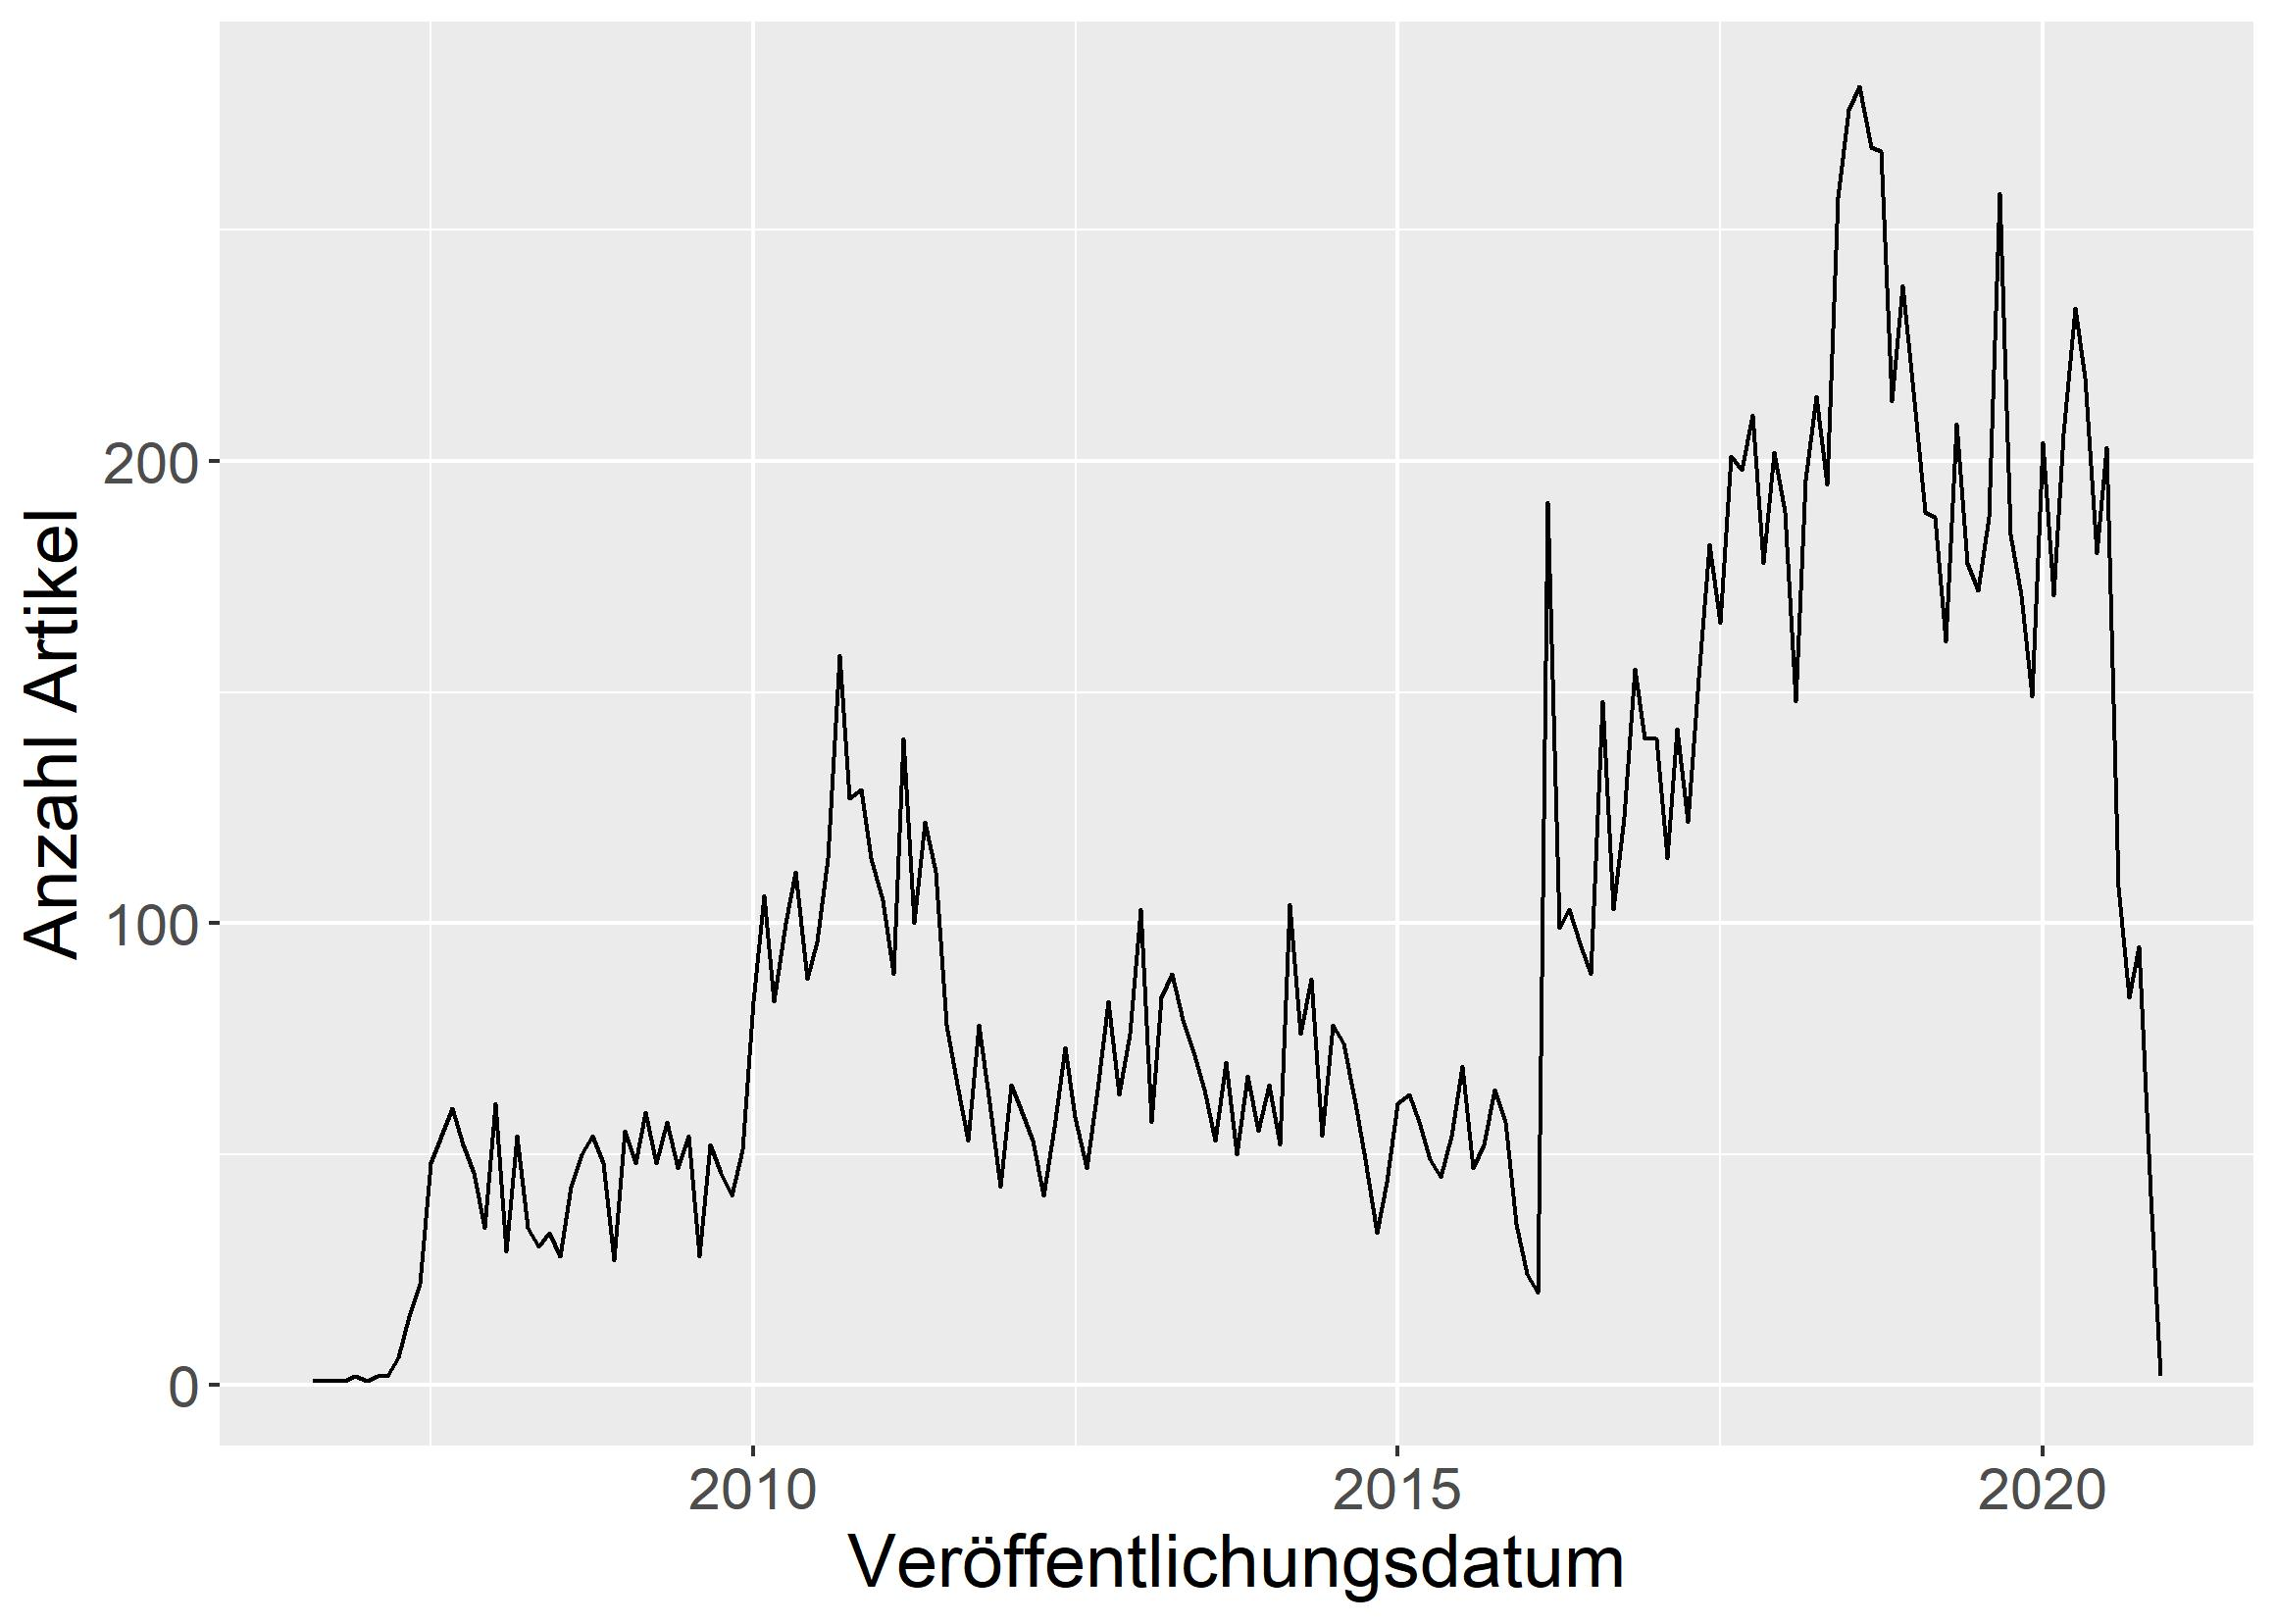
\includegraphics[scale=0.45]{graphics/cons_freq_time.jpg}
    \caption{Anzahl Artikel nach Veröffentlichungsdatum (nach Monat gruppiert)}
    \label{article-frequency}
\end{figure}

Der so erstellte Korpus umfasst ingsgesammt 16836 Texte und deckt beginnend in 2006 einen Zeitraum von 14 Jahren ab.
Wie in Grafik \ref{article-frequency} zu erkennen ist, steigt beginnend in 2016 die Zahl der Artikel im Korpus deutlich an.
\todo{Wirklich?}
Dies liegt zum einen daran, dass einzelne der betrachteten Angebote die Veröffentlichungsfrequenz erhöhrt haben, ist aber überwiegend darauf zurückzuführen, dass nicht alle Internetangebote über den gesammten Zeitraum existiert haben sondern erst später aktiv wurden.
Genauere Informationen zu den von den einzelnen Angeboten abgedeckten Zeiträumen sowie zu Artikelzahl und Länge finden sich in Tabelle \ref{corpus-stats}.

Wie dort auch ersichtlich ist, unterscheidet sich nicht nur die absolute Zahl der Artikel nach Quelle stark, auch das Veröffentlichungsinterval schwankt von weniger als einem Artikel den Monat bis über 100.
Es besteht weiterhin ein negativer Zusammenhang zwischen der Artikellänge und dem Veröffentlichungsintervall (\todo{r richtiges Zeichen?}$r = -0.72, p = 0.065$).

\begin{table}
    \begin{center}
        \begin{tabularx}{\textwidth}{lXXXXX}
            \toprule
            & Von & Bis & Mittlere Zeichenzahl & Anzahl Artikel & Artikel/Monat\\
            \midrule
            Alles Schall und Rauch & 23.08.2006 & 02.08.2020 & 5000 & 5349 & 32.0\\
            conrebbi & 05.09.2012 & 20.10.2014 & 5610 & 24 & 1.0\\
            deutschlandpranger & 29.10.2016 & 30.12.2020 & 7527 & 118 & 2.4\\
            fm-tv & 31.07.2008 & 02.11.2018 & 9158 & 97 & 0.8\\
            hinterderfichte & 16.01.2010 & 31.05.2018 & 4221 & 1083 & 10.8\\
            \addlinespace
            recentr & 03.08.2007 & 05.08.2020 & 5071 & 4762 & 30.5\\
            Watergate.tv & 20.05.2016 & 16.11.2020 & 2810 & 5403 & 101.9\\
            \bottomrule
            \end{tabularx}
        \caption{Kennzahlen der einzelnen Quellen des Korpuses}
        \label{corpus-stats}
    \end{center}
\end{table}

Auch eine inhaltliche Betrachtung zeigt deutliche Unterschiede zwischen den einzelnen Angeboten.
So ist etwa \textit{Alles Schall und Rauch} (\textit{ASuR}) als ältestes vertretenes Angebot auch einer der "klassischsten" \todo{Das muss anders} Vertreter des Genres.
Hier wird der Nutzer direkt auf der Startseite mit Fragen konfrontiert wie "Was geschau wirklich am 11. September?" oder "Was passiert tatsächlich mit dem Klima?" \parencite{asur-homepage}. \todo{Eventuell zitation zu häufigen fragen.}

Die Seite bedient sich klassischer Verschwörungstheorien und wird im allgemeinen der Truther Szene zugeordnet \parencite{psiram-asur}.
Sie hat laut eigenaussage im Schnitt über 50.000 Zugriffe täglich\footnote{Der Besucherzähler der Website ist inzwischen nicht mehr funktional, Angabe übernommen aus \parencite{vice-asur}}.

Inhaltlich finden sich sowohl Essay-artige Artikel zu Themen wie 9/11, Bilderberger oder Klimawandel auf der Seite, als auch kürzer gehaltene Meldungen zu aktuellen Ereignissen.
Es werden, wie bei fast allen anderen Seiten im Korpus, häufig Inhalte Dritter eingebunden sowie die Artikel durch Bilder oder Grafiken ergänzt.

Ähnlich gelagert sind die Angebote \textit{Hinter der Fichte} (\textit{HdF}) und \textit{conrebbi}, beide können der Truther Szene zugerechnet werden (siehe etwa \cite{psiram-conrebbi}).
In beiden Angeboten werden aktuelle Ereignisse kommentiert und verschwörungstheoretisch interpretiert, sowie längere Essays zu typischen Themen verfasst.
Im Vergleich zu \textit{ASuR} werden bei beiden Angeboten deutlich mehr Inhalte in Form von Videos und Fremdquellen in Bild und Textform genutzt.

Etwas aus der Reihe fallen die Angebote \textit{fm-tv} sowie \textit{Deutschlandpranger}.
Inhaltlich finden sich etwa beim \textit{Deutschlandpranger} recht klassische Themen wie die Leugnung des Klimawandels \parencite*[vgl.][]{dprang-klima}, sind die dazugehörigen Text überdurchschnittlich lang und voller Werbung für Bücher zu z.T. komplett unabhängigen Themen.
Auch sind die Texte selbst teilweise relativ wirr, so enthalten beispielsweise die (sehr ausführlichen) AGB einen Abschnitt zu Strafzahlungen bei "Übersenden eines Statements anstatt einer echten Rechnung (True Bill) des wahren Haftungsgläubigers" \parencite*{dprang-agb}.

Die verbleibenden beiden Angebote \textit{recentr} und \textit{Watergate.tv} sind beide der rechten Szene zuzuordnen und verbreiten Verschwörungstheorien in diese Richtung.
Beide zeichnet ein eher journalistischer Stil aus, es werden kurze bis mittellange Meldungen veröffentlicht, häufig begleitet von eigenen oder fremden Videos.
\textit{Recentr} wurde 2006 als deutscher Ableger von \textit{Inforwars.com} gegründet und bedient sich noch heute einem ähnlichen Konzept.
Ähnlich dem Vorbild wird massiv Werbung für den eigenen Shop gemacht in dem diverse Produkte zur Vorbereitung auf apokalyptische Szenarien sowie fragwürdige Nahrungsergänzungsmittel verkauft werden.
Inhaltlich ist vor allem interessant, dass sich die Seite (bzw. der Hauptautor Alexander Benesch) z.T. sehr explizit von anderen Teilen der rechten/verschwörungstheoretischen Szene abgrenzt.
\footnote{So grenzt sich das Portal in Beiträgen inzwischen auch von \textit{Inforwars} Gründer Alex Jones ab \parencite*{recentr-jones} oder spekuliert darüber, ob die Alternative für Deutschland vom britischen Geheimdienst gegründet wurde \parencite{recentr-afd}}
So kommt es durchaus vor, dass in einem Artikel zunächst von der "implausiblen Sichtweise, verschiedenste Regierungen hätten eine Fake-Pandemie orchestriert" \parencite{recentr-population} gesprochen wird, nur um im nächsten Satz zu erklären: 

\begin{quotation}
    In Wirklichkeit sind die Methoden der globalen Bevölkerungsreduktion fast ausschließlich legal, simpel und werden schrittweise angewandt [...]. Das Konzept ist so entworfen, um mit möglichst wenig Zwang auszukommen [...]. \parencite{recentr-population}
\end{quotation} 

Die Website \textit{Watergate.tv} (inzwischen Teil von \textit{NEOPresse.com}) ist ein rechtslastiges Nachrichten und Videoportal, das sich verschwörungstheoretischer Narrative bedient. 
Auf dem Portal finden sich klassische Themen wie Bilderberger \parencite[vgl.][]{watergate-bilderberger} aber auch Fake-News und Berichterstattung mit starker pro-russischen Tendenz.
In die öffentlichkeit Rückte das Portal als sich das Neo-Magazin-Royale wegen seiner Mitarbeit bei \textit{Watergate.tv} von Hans Meiser trennte \parencite*[Siehe z.B.][]{spiegel-watergate}.

\todo{Kurzes Fazit Korpus}

% Vergleichskorpus

Bei der Erstellung des Vergleichskorpus war es das Ziel Quellen zu wählen die dem Korpus konspirativer Texte möglichst ähnlich sind, ohne die konspirativen Aspekte zu enthalten.
Da insbesondere die letzten beiden besprochenen Angebote sich inhaltlich sehr an journalisitsche Angebote anlehnen, lag es nah ebensolche heranzuziehen.
Aus Gründen der Vollständigkeit (Die Angebote sollten möglichst den kompletten Zeitraum des Korpuses abdecken) sowie der Zugänglichkeit wurden die Angebote von Spiegel Online sowie der Frankfurter Rundschau ausgewählt.
Es wurde für beide Onlineangebote zunächst ein Index aller Artikel die in den selben Zeitraum wie der Korpus fallen erstellt und aus diesem zufällig eine Auswahl von 10000 Artikeln pro Anbieter gezogen.

Die restlichen im Korpus enthaltenen Seiten sind alle mehr oder weniger in Blogform gehalten.
Um Inhalte in einer vergleichbaren Form zu findne aber auch dem in der Literatur häufig anzutreffenden Feststellungen der wissenschaftlichen Form von verschwörungstheoretischen Texten Rechnung zu tragen wurde eine Reihe von Wissenschaftsblogs als zweite Komponente im Vergleichskorpus gewählt.
Dafür wurden von den beiden Platformen scienceblogs und scilogs\footnote{Beide Platformen sind Anbieter bei denen eine Vielzahl verschiedener Blogs zu finden sind.} ähnlich den journalistischen Angeboten aus dem gesamten Index der Einträge eine Auswahl von jeweils 10000 Artikeln ausgewählt.
Genauere Kennwerte zum Vergleichskorpus siehe in Tabelle \ref{comcorpus-stats}.

\begin{table}
    \begin{center}
        \begin{tabularx}{\textwidth}{XXXXXX}
            \toprule
            & Von & Bis & Mittlere Zeichenzahl & Anzahl Artikel & Artikel/Monat\\
            \midrule
            Frankfurter Rundschau & 03.08.2006 & 04.08.2020 & 3670 & 9959 & 59.3\\
            scienceblogs & 14.02.2007 & 04.08.2020 & 3261 & 8765 & 54.4\\
            scilogs & 29.12.2000 & 03.08.2020 & 5206 & 9533 & 40.6\\
            Spiegel Online & 01.08.2006 & 07.01.2020 & 4687 & 8665 & 53.8\\
            \bottomrule
        \end{tabularx}
        \caption{Kennzahlen der einzelnen Quellen des Vergleiskorpuses}
        \label{comcorpus-stats}
    \end{center}
\end{table}

\subsection{Datenvorverarbeitung}

Zunächst wurden einige Säuberungsschritte auf den Korpus angewendet, um zu verhindern, dass fehlerhafte oder irrelevante Daten mit für die Feature Erstellung herangezogen werden.

Es wurde zunächst Unicode Normalisierung für alle Texte durchgeführt, anschließend wurden mittels des \textit{Google Compact Language Detector 3} \parencite[][]{cld3} die Sprache aller Text bestimmt nur (überwiegend) deutschsprachige Texte zu betrachten.
Da im Korpus an einigen Stellen noch nicht zum Artikeltext gehörige Komponenten aus vielen Sonderzeichen vorhanden waren, wurden alle Wörter entfernt, die nur aus Zeichen bestanden, die unter 1000 Mal im gesammten Korpus vorkamen.
Schlussendlich wurden noch kleinere Korrekturen vorgenommen, wie das Zusammenfassen multipler, aufeinanderfolgender Leerzeichen und Unterstriche (die gerne als Trennlinien in den Text benutzt wurden).

Schlussendlich wurden noch alle Text unter 100 Zeichen länge aus dem Korpus entfernt, da diese für die Klassifizierungsaufgabe nur wenig Informationen enthalten können. Der finale Korpus umfasste 53758 Texte, mit einem Anteil der positiven Klasse (sprich von verschwörungstheoretischen Texten) von etwa 32\%.

\subsection{Feature Erstellung}

